\documentclass[10pt,twocolumn,letterpaper]{article}

\usepackage[utf8]{inputenc}
\usepackage[margin=0.75in]{geometry}
\usepackage{times}
\usepackage{microtype}
\usepackage{graphicx}
\usepackage{booktabs}
\usepackage{amsmath}
\usepackage{amssymb}
\usepackage{hyperref}
\usepackage{xcolor}
\usepackage{cite}
\raggedbottom

\hypersetup{
    colorlinks=true,
    linkcolor=blue,
    citecolor=blue,
    urlcolor=blue
}

\title{\textbf{Constitutional Grounding vs. Dynamic Skill Loading:\\An Empirical Evaluation of Autonomous Agents in Terminal Environments on Terminal-Bench 2.1}}

\author{
  \textbf{Utkarsh Chandra}\thanks{Project repository, evaluation harness, and verification artifacts: \url{https://github.com/Utkarsh-X/Supreme}}\\
  \textit{The Supreme Project}
}

\date{}

\begin{document}

\twocolumn[
  \begin{@twocolumnfalse}
    \maketitle
    \begin{abstract}
Autonomous software engineering agents operating in terminal environments are increasingly tasked with complex debugging, systems administration, and algorithmic workflows. A central architectural consideration in agent design is how guidance is structured: embedding invariant engineering principles directly within the initial context versus dynamically loading specialized procedural skills on demand. In this work, we compare the behavior of three substantially different agent-guidance configurations across all 89 tasks of the official Terminal-Bench 2.1 benchmark (267 isolated container evaluations) using Gemini 3.6 Flash High within a unified evaluation harness: Supreme (an invariant constitutional framework), a dynamic skill-loading system based on Superpowers by obra (\texttt{obra/superpowers}), and an unprompted baseline. Across the full benchmark, Supreme achieved the highest task completion (61/89, 68.5\% vs.\ 58/89, 65.2\% for Superpowers and 55/89, 61.8\% for Baseline; 70.9\% vs.\ 67.4\% vs.\ 64.0\% after adjusting for upstream container defects), the lowest aggregate wall-clock runtime (15.15h vs.\ 18.30h and 16.92h), and the lowest effective paid cost per successful task (\$0.489, approximately 3.4\% below Superpowers at \$0.506). While aggregate accuracy differences across the 89 tasks are not statistically distinguishable under paired McNemar tests ($p > 0.05$) and instruction content remains coupled with delivery mechanisms, the configurations exhibit distinct behavioral and economic profiles. On Hard tasks ($N=30$), Supreme demonstrated an increase in provider-reported deliberation tokens (+66.0\%, from 17.0k to 28.3k thinking tokens/task) alongside a directional pass-rate lead (66.7\% vs.\ 53.3\%; paired McNemar $p = 0.22$, exact binomial $p = 0.22$). Transcripts reveal stark operational failure modes: in open-ended combinatorial tasks (e.g., Task \#88), unconstrained dynamic skill exploration coincided with extensive script-generation loops, writing 116 exploratory files and consuming 3.51 million tokens ($11.7\times$ the tokens of Supreme's 300k-token solve). Furthermore, context-growth accounting indicates that frequent on-demand documentation ingestion accumulated 411.3 million cache read tokens (+115.4 million over baseline). We provide complete execution transcripts, evaluation harness configurations, and cryptographic audit ledgers to facilitate independent replication.
\end{abstract}


    \vspace{0.8em}
  \end{@twocolumnfalse}
]
{
  \renewcommand{\thefootnote}{\fnsymbol{footnote}}
  \footnotetext[1]{Project repository, evaluation harness, and verification artifacts: \url{https://github.com/Utkarsh-X/Supreme}}
}

\section{Introduction}
\label{sec:intro}

The deployment of frontier large language models as autonomous agents in real-world software engineering and systems administration requires navigating complex, stateful terminal environments \cite{shaw2025terminalbench, jimenez2024swebench}. Unlike single-turn question-answering or isolated code generation benchmarks, terminal-grounded tasks demand sustained multi-turn reasoning, file system traversal, compiler diagnostics, and iterative error recovery \cite{yao2023react, google2026gemini36}.

As agent systems scale in complexity, a central architectural question is how operational capabilities, procedural guidance, and behavioral constraints should be structured:
\begin{enumerate}\itemsep0pt \parskip0pt \parsep0pt
    \item \textbf{Dynamic Progressive Skill Loading}: Exemplified by modular agent frameworks such as \textit{Superpowers by obra} \cite{vincent2025superpowers}, this design aims to keep initial prompt context compact by exposing a lightweight capability catalog. The agent discovers relevant skills (e.g., test-driven development, systematic debugging, git worktrees) and loads procedural guidance on demand.
    \item \textbf{Constitutional Static Grounding}: The Supreme configuration draws on constitutional principles \cite{bai2022constitutional} and embeds invariant engineering rules (evidence-over-assumption, targeted edits, hierarchical decomposition, and loop management) in its static system-prompt header.
\end{enumerate}

An earlier exploratory evaluation on a simpler 50-task subset (CARB-v2) yielded high pass rates: 94\% for Baseline, 94\% for Supreme, and 92\% for Superpowers. The reported aggregate comparison was not statistically distinguishable (paired McNemar $p = 1.0$), leaving limited headroom to distinguish outcomes on that subset. We therefore evaluate the complete 89-task Terminal-Bench 2.1 corpus, which covers systems administration, multi-stage compilation, and low-level kernel emulation.

We compare three complete configurations---Supreme, Superpowers by obra, and an unprompted baseline---across the 89 Terminal-Bench 2.1 tasks (267 container evaluations), using Gemini 3.6 Flash High within a shared evaluation harness. The central question is how these configurations compare in task completion, execution economics, and behavior under the same model, harness, and benchmark. This first iteration establishes an empirical baseline for replication and future controlled ablations.

Because Supreme and Superpowers differ in both guidance delivery and instructional content, this comparison does not isolate either factor.

Our investigation yields four primary contributions:
\begin{itemize}
    \item \textbf{Hard-Task Deliberation Patterns}: Supreme's mean provider-reported deliberation tokens increased by 66.0\% from Medium to Hard tasks. On Hard tasks, Supreme passed 20/30 compared with 16/30 for Superpowers (paired McNemar $p = 0.22$), a directional difference that does not establish a causal link between deliberation-token use and task success.
    \item \textbf{Task 88 Case Study}: Both runs passed; Superpowers used 3.51M tokens over 563 turns versus 0.30M over 55 turns for Supreme.
    \item \textbf{Multi-Turn Context Accounting and Cache Telemetry}: Provider telemetry recorded 411.3 million cache-read tokens for Superpowers, compared with 322.8 million for Supreme and 295.9 million for Baseline. These observed totals do not isolate how much of the difference is attributable to dynamically loaded documentation.
    \item \textbf{Polyglot Domain Breakdown and Esoteric \& Symbolic Tasks}: Across five engineering domains, Supreme recorded the highest pass rates in Low-Level Systems and SysAdmin \& DevOps, while the unprompted Baseline recorded the highest rate in the Esoteric \& Symbolic domain (85.7\%), which includes COBOL and Scheme tasks.
\end{itemize}


\section{Related Work}
\label{sec:related_work}

\textbf{Autonomous Software Engineering Benchmarks.} 
Early LLM coding benchmarks such as HumanEval and MBPP evaluated isolated functions using synthetic unit tests. SWE-bench \cite{jimenez2024swebench} introduced real-world GitHub issues requiring repository navigation and code changes. Terminal-Bench 2.1 \cite{shaw2025terminalbench} complements this focus with interactive, multi-container Linux tasks involving shell use, package compilation, daemon orchestration, and runtime debugging.

\textbf{Agent Prompt Architectures.}
The foundational ReAct framework \cite{yao2023react} interleaves chain-of-thought reasoning traces with action execution. Subsequent research has explored dynamic capability adaptation, such as Toolformer \cite{schick2024toolformer}, which trains models to invoke APIs on demand. In open-source agent ecosystems, progressive skill-loading systems have emerged. \textit{Superpowers by obra} \cite{vincent2025superpowers} formalizes progressive disclosure, enabling agents to discover and read structured procedural skills from disk, with the aim of keeping initial prompt context compact.

\textbf{Constitutional AI and Guardrails.}
Constitutional AI \cite{bai2022constitutional} studies alignment through explicit principles that guide model behavior. The Supreme configuration applies engineering rules in its static prompt context---including targeted edits, hypothesis-driven debugging, and verification before completion---with the aim of guiding coding agents toward bounded, verifiable actions.

\textbf{Prompt Caching and Multi-Turn Context Use.}
Model APIs offer prompt caching \cite{anthropic2024promptcaching, google2026gemini36}, which can reduce the cost and latency of repeated context prefixes. Prefix caching generally depends on stable matching prefixes. Changes to agent context, such as inserted skill documents, large file dumps, or tool-schema updates, may affect cache reuse. This study reports provider-reported cache-read totals across three configurations in multi-turn terminal tasks; it does not isolate the effect of any one context change.


\section{Agent System Architectures}
\label{sec:architectures}

To strictly isolate the impact of prompt and systems architecture from foundation model variance, all three paradigms were evaluated using the identical underlying foundation model engine (\texttt{gemini-3.6-flash-high}) at zero temperature ($\tau=0.0$), with identical tool schemas for shell execution, file reading, file editing, and process management.

\subsection{Supreme (v1.0): Constitutional Static Grounding}
Supreme v1.0 structures agent behavior through a static, invariant constitutional framework permanently positioned in the system prompt header. It consists of five core operational modules:
\begin{itemize}
    \item \textbf{Engineering Constitution}: Invariant behavioral axioms prioritizing directly verifiable evidence over model assumption, user intent preservation, and proportional scrutiny scaling with action blast radius.
    \item \textbf{Operating Protocol}: A decision framework enforcing four sequential execution phases: intent extraction, hierarchical decomposition, surgical code modification, and multi-signal verification.
    \item \textbf{Surgical Editing Mandate}: Explicit diff constraints requiring agents to justify line changes, use targeted line-replacement tools (\texttt{replace\_file\_content}), and strictly avoid opportunistic or cosmetic file rewrites.
    \item \textbf{Anti-Premature-Closure}: A mandatory verification forcing function requiring agents to ask: \textit{"If this implementation were falsely claiming completion, what plausible omission was overlooked?"}
    \item \textbf{Loop Management Protocol}: Hard limits on consecutive failing commands and strict prohibitions against passive background task polling loops.
\end{itemize}
Under this architecture, the system prompt prefix of length $L_{\text{const}} \approx 4,800$ tokens remains strictly invariant across all turns $t \in [1, T]$, ensuring deterministic prefix cache hits on every interaction turn.

\subsection{Superpowers by obra: Dynamic Progressive Skill Loading}
Superpowers by obra \cite{vincent2025superpowers} implements two-tier progressive capability disclosure. The initial system prompt contains a compact index summarizing 14 distinct engineering skills:
\begin{enumerate}
    \item \texttt{using-superpowers} (Meta-discovery \& catalog dispatch)
    \item \texttt{systematic-debugging} (Root-cause tracing and defense-in-depth)
    \item \texttt{test-driven-development} (Red-Green-Refactor TDD cycle)
    \item \texttt{writing-plans} (Hierarchical multi-phase execution planning)
    \item \texttt{executing-plans} (Systematic plan fulfillment and checkpointing)
    \item \texttt{verification-before-completion} (Pre-flight validation gates)
    \item \texttt{subagent-driven-development} (Isolated task delegation)
    \item \texttt{requesting-code-review} (Pre-commit review requests)
    \item \texttt{receiving-code-review} (Critique integration and refactoring)
    \item \texttt{finishing-a-development-branch} (Merge sanitation and branch cleanup)
    \item \texttt{dispatching-parallel-agents} (Concurrent sub-agent dispatch)
    \item \texttt{using-git-worktrees} (Isolated filesystem branching)
    \item \texttt{brainstorming} (Design exploration and architecture ideation)
    \item \texttt{writing-skills} (Dynamic procedural skill creation)
\end{enumerate}
When an agent determines that a skill is required, it dynamically invokes file-reading tools to ingest the corresponding \texttt{SKILL.md} and nested reference documents into the conversational history. While reducing the initial prompt to $\approx 1,200$ tokens, this on-demand injection inserts reference text directly into the active dialogue turns.

\subsection{Baseline: Unprompted Control}
The Baseline configuration provides the raw LLM engine with execution capabilities and tool declarations, but omits all auxiliary system instructions, behavioral protocols, and skill catalogs. It serves as the empirical control to measure the baseline competence of the underlying model.

\subsection{Methodological Scope: Structure vs.\ Content}
We emphasize that Supreme and Superpowers differ along two dimensions simultaneously: structural delivery (static invariant prompt header vs.\ on-demand dynamic disk retrieval) and semantic instruction content (constitutional axioms and surgical diff boundaries vs.\ procedural engineering recipes such as TDD and worktrees). Consequently, the empirical results presented in this work reflect the overall behavior of the complete configurations. Controlled ablations (e.g., statically injecting Superpowers documentation, or applying constitutional loop controls to dynamic skill loading) will be valuable in future work to cleanly decouple delivery mechanisms from prompt semantics.



\section{Experimental Setup}
\label{sec:setup}

\subsection{Benchmark Corpus: Terminal-Bench 2.1}
We evaluate across the complete 89-task corpus of Terminal-Bench 2.1 \cite{shaw2025terminalbench}. To analyze real-world polyglot versatility beyond standard Python scripting, we classify all 89 tasks across five distinct technical engineering stacks:
\begin{itemize}
    \item \textbf{Low-Level \& Systems Engineering} ($N=20$): C, C++, x86/ARM/MIPS Assembly, Redcode, Rust, and OCaml compiler runtimes.
    \item \textbf{SysAdmin, OS \& DevOps} ($N=15$): Linux kernel parameters, QEMU hypervisor orchestration, Git object reconstruction, OpenSSH, and Bind9 DNS.
    \item \textbf{Software Engineering} ($N=26$): Python applications, Cython extensions, complex data pipelines, and multi-file refactors.
    \item \textbf{Esoteric \& Symbolic Programming} ($N=14$): Scheme metacircular evaluators, COBOL business logic, LaTeX typesetting, Stan probabilistic modeling, and SPARQL ontology queries.
    \item \textbf{Machine Learning \& Robotics} ($N=14$): PyTorch distributed parallelism, HuggingFace transformers, FastText embeddings, and MuJoCo XML physics modeling.
\end{itemize}

\subsection{Evaluation Isolation and Anti-Leakage Protocol}
To ensure benchmark validity and prevent evaluation leakage during task execution, the evaluation harness enforces strict multi-container isolation:
\begin{enumerate}
    \item \textbf{Pristine Container Provisioning}: An isolated Docker container is spawned from the official benchmark image with bounded memory and CPU allocations.
    \item \textbf{Evaluation Isolation}: During active agent problem-solving, the ground-truth verification suite (\texttt{/tests}) is absent from the container filesystem. The captured run logs record 104 exploratory shell searches attempting to locate verification files (e.g., \texttt{find / -name "*test*"}); all recorded attempts returned empty results. This indicates that agents did not access ground-truth tests through these searches, though it does not preclude pre-training data exposure.
    \item \textbf{Per-Task Timeout Enforcement}: Each task operates under its official per-task timeout $T_{\text{limit}}$ specified in its benchmark configuration (\texttt{task.toml}). Across the corpus, timeouts range from 600s to 12,000s with a median of 900s ($49$ of $89$ tasks at the median). Heavy systems and simulation tasks (e.g., \texttt{install-windows-3.11} and \texttt{winning-avg-corewars}) are allocated 3,600s. Upon self-declaration of completion or reaching $T_{\text{limit}}$, the agent process tree is terminated. Recorded wall-clock includes session teardown: 37 of 267 runs exceeded $T_{\text{limit}}$ (36 by at most 39\,s of teardown); one anomalous baseline session (\texttt{merge-diff-arc-agi-task}, 7{,}035\,s vs.\ a 900\,s limit) is flagged in the audit ledger.
    \item \textbf{Post-Execution Injection}: The official verifier is copied into the container via \texttt{docker cp tests/ container:/tests} only after agent execution has completed.
    \item \textbf{Multi-Signal Consensus Verification}: An isolated subshell executes \texttt{test.sh}, capturing binary reward status, individual CTRF unit test counts, and raw terminal stdout/stderr logs.
    \item \textbf{Cryptographic Audit Trail}: A SHA-256 hash is computed over all verifier artifacts and committed to the audit ledger.
\end{enumerate}

\subsection{Telemetry and Token Accounting}
For runs with successfully captured turn streams, token metrics are extracted from provider API response metadata on each turn:
\begin{itemize}
    \item \textbf{Input Tokens ($T_{\text{in}}$)}: Total prompt tokens presented to the model per turn.
    \item \textbf{Cache Read Tokens ($T_{\text{cache}}$)}: Prompt tokens retrieved from provider-side prefix cache (\texttt{cached\_content\_token\_count}).
    \item \textbf{Deliberation Tokens ($T_{\text{think}}$)}: Provider-reported reasoning tokens generated during internal model deliberation (\texttt{thinking\_tokens}), captured as aggregate counts rather than decoded chain-of-thought text.
    \item \textbf{Output Tokens ($T_{\text{out}}$)}: Generated text and tool-call payload tokens (\texttt{candidates\_token\_count}).
\end{itemize}

Aggregate recorded token totals are calculated from the captured input and output usage fields. Deliberation tokens are shown separately for analysis and are already included in the output total. The canonical Task~\#44 (\texttt{mailman}) records for Superpowers and Baseline contain a 350,000-token placeholder but no captured turn-level usage; these placeholders are excluded, and no values are imputed for the missing usage.


\section{Empirical Results}
\label{sec:results}

Across all 89 tasks (267 isolated container evaluations), Supreme achieved the highest task completion (61/89, 68.5\%), the lowest aggregate wall-clock time (15.15\,h), and the lowest effective evaluation cost per successful task under recorded OpenRouter rates (\$0.489, approximately 3.4\% below Superpowers at \$0.506). Figure~\ref{fig:macro_summary} provides an executive visual comparison; Table~\ref{tab:master_scoreboard} details the complete scoreboard including infrastructure-adjusted cohorts ($N=86$, $N=85$).

\begin{table*}[t]
\centering
\caption{CARB-v4 Master Scoreboard across all 89 Terminal-Bench 2.1 tasks on Gemini 3.6 Flash High. Brackets denote Wilson 95\% score confidence intervals. Adjusted scores exclude three tasks with verified upstream container environment defects ($N=86$); a further conservative cohort excluding all four infrastructure-impaired tasks ($N=85$) is reported in Section~\ref{sec:case_studies}.}
\label{tab:master_scoreboard}
\resizebox{\textwidth}{!}{%
\begin{tabular}{lccccccc}
\toprule
\textbf{Configuration} & \textbf{Raw Solved} & \textbf{Raw Pass (\%)} & \textbf{Adjusted Pass (\%)} & \textbf{Total Time (h)} & \textbf{Avg Time / Task (s)} & \textbf{Total Tokens} & \textbf{Tokens / Solved} \\
\midrule
\textbf{Supreme} & \textbf{61 / 89} & \textbf{68.5\%} [58.3\%, 77.2\%] & \textbf{70.9\% (61/86)} [60.6\%, 79.5\%] & \textbf{15.15} & \textbf{612.9} & 34,521,410 & \textbf{565,925} \\
Superpowers by obra & 58 / 89 & 65.2\% [54.8\%, 74.3\%] & 67.4\% (58/86) [57.0\%, 76.4\%] & 18.30 & 740.2 & 34,304,008 & 591,448 \\
Baseline & 55 / 89 & 61.8\% [51.4\%, 71.2\%] & 64.0\% (55/86) [53.4\%, 73.3\%] & 16.92 & 684.3 & \textbf{31,217,863} & 567,598 \\
\bottomrule
\end{tabular}%
}
\end{table*}

\subsection{Macro Accuracy and Statistical Significance}
Supreme achieved 61 verified wins (68.5\%), compared to 58 (65.2\%) for Superpowers by obra (+3 wins) and 55 (61.8\%) for Baseline (+6 wins).

To test whether aggregate pass rate differences are statistically distinguishable, we conducted paired McNemar's tests with Edwards' continuity correction. Comparing Supreme vs.\ Superpowers yields 52 mutual passes, 22 mutual failures, 9 Supreme-only wins, and 6 Superpowers-only wins ($\chi^2 = 0.267, p = 0.605$). Comparing Supreme vs.\ Baseline yields 12 Supreme wins vs.\ 6 Baseline wins ($\chi^2 = 1.389, p = 0.239$). Comparing Superpowers vs.\ Baseline yields 12 Superpowers-only wins and 9 Baseline-only wins ($\chi^2 = 0.190, p = 0.663$).

These paired tests confirm that aggregate pass rates do not differ significantly across architectures ($p > 0.05$). The primary empirical findings emerge not from gross accuracy margins, but from operational differences in \textbf{deliberation scaling, tool ecology, and context economics}.

\begin{figure*}[t]
\centering
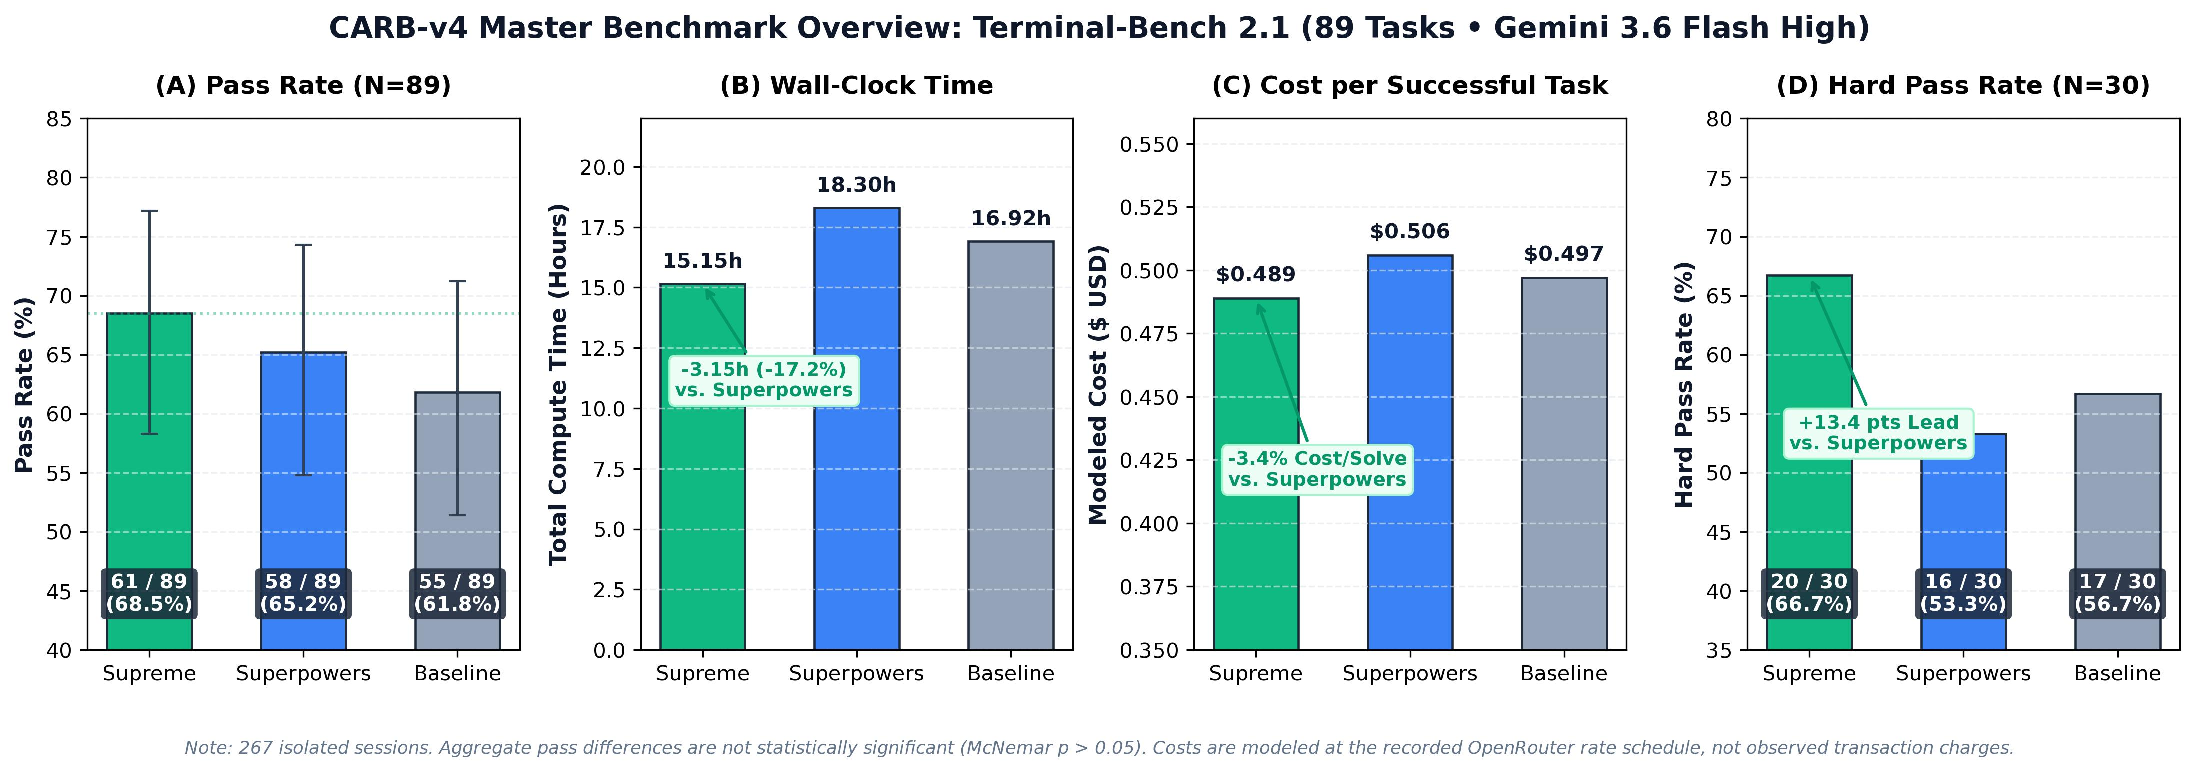
\includegraphics[width=0.98\textwidth]{figures/macro_benchmark_summary.pdf}
\caption{Benchmark outcomes and execution efficiency across all 89 Terminal-Bench 2.1 tasks (267 graded container evaluations). (A) Task completion rates with Wilson 95\% confidence intervals. (B) Total wall-clock execution time (lower is better). (C) Effective evaluation cost per successful task under recorded OpenRouter rates (lower is better). (D) Hard-task frontier pass rates ($N=30$). Supreme achieved the highest task completion (61/89, 68.5\%), the lowest aggregate wall-clock time (15.15\,h, 17.2\% lower than Superpowers), and the lowest effective evaluation cost per successful task under recorded OpenRouter rates (\$0.489, approximately 3.4\% below Superpowers). Aggregate accuracy differences are not statistically significant under paired McNemar tests ($p > 0.05$); see Section~\ref{sec:results} for full statistical analysis.}
\label{fig:macro_summary}
\end{figure*}


\subsection{Deliberation Scaling Patterns by Task Difficulty}
Across the 267 executions, the model generated 5,311,737 provider-reported deliberation tokens (\texttt{thinking\_tokens}). Table~\ref{tab:difficulty_scaling} disaggregates pass rates and mean deliberation tokens across official difficulty tiers.

\begin{table}[h]
\centering
\caption{Deliberation and Win Rates Across Complexity Strata (Wilson 95\% CIs in brackets).}
\label{tab:difficulty_scaling}
\resizebox{\columnwidth}{!}{%
\begin{tabular}{llccc}
\toprule
\textbf{Strata} & \textbf{Metric} & \textbf{Supreme} & \textbf{Superpowers} & \textbf{Baseline} \\
\midrule
\textbf{Easy} & Pass Rate & \textbf{75.0\% (3/4)} [30.1, 95.4] & 25.0\% (1/4) [4.6, 69.9] & 50.0\% (2/4) [15.0, 85.0] \\
($N=4$) & Mean Deliberation & 11,885 & 14,618 & 10,688 \\
\midrule
\textbf{Medium} & Pass Rate & 69.1\% (38/55) [56.0, 79.7] & \textbf{74.5\% (41/55)} [61.7, 84.2] & 65.5\% (36/55) [52.3, 76.6] \\
($N=55$) & Mean Deliberation & 17,035 & 17,350 & 18,090 \\
\midrule
\textbf{Hard} & Pass Rate & \textbf{66.7\% (20/30)} [48.8, 80.8] & 53.3\% (16/30) [36.1, 69.8] & 56.7\% (17/30) [39.2, 72.6] \\
($N=30$) & Mean Deliberation & \textbf{28,271} & 23,196 & 24,426 \\
\bottomrule
\end{tabular}%
}
\end{table}

Due to the small Easy strata ($N=4$), pass rates in that tier carry wide confidence intervals and are reported for completeness; no comparative inference should be drawn from them.

On Hard tasks ($N=30$), Supreme scaled mean deliberation by +66.0\% over Medium tasks (from 17.0k to 28.3k thinking tokens/task; Table~\ref{tab:difficulty_scaling}), achieving a 66.7\% pass rate (20/30). In contrast, Superpowers generated 23,196 thinking tokens/task with a 53.3\% pass rate (16/30). 

To examine this difference statistically on the Hard subset, we constructed the paired $2 \times 2$ contingency table for Supreme vs.\ Superpowers: 15 mutual passes, 9 mutual failures, 5 Supreme-only wins, and 1 Superpowers-only win. A paired McNemar test with continuity correction yields $\chi^2 = 1.500, p = 0.221$ (exact two-tailed binomial $p = 0.219$). Because this 4-task margin does not attain significance at $\alpha = 0.05$, we characterize this as a suggestive behavioral pattern (McNemar $p = 0.22$) rather than a confirmed scaling law. In Section~\ref{sec:case_studies}, we examine transcripts to investigate how dynamic documentation ingestion interacted with reasoning on these tasks.

\begin{figure*}[t]
\centering
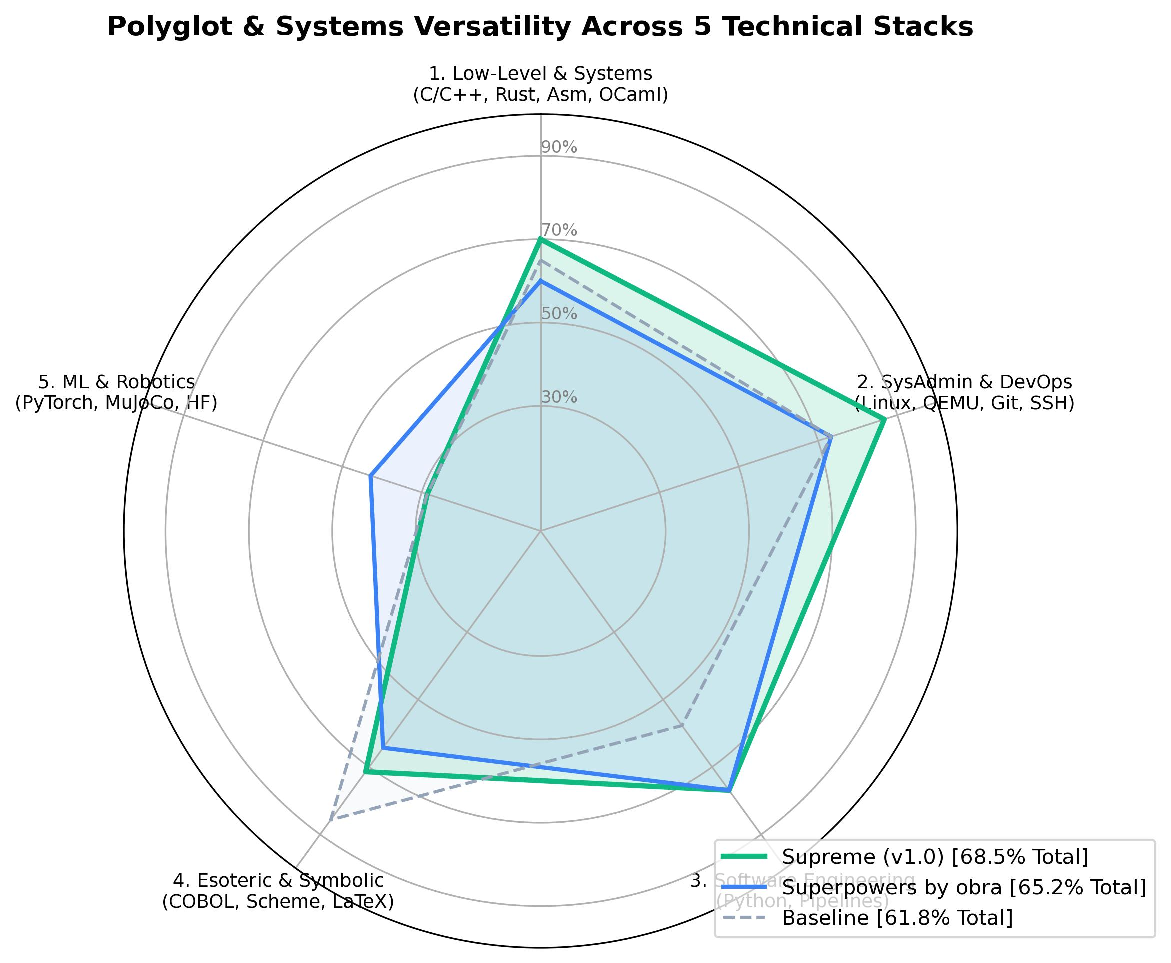
\includegraphics[width=0.48\textwidth]{figures/fig3_polyglot_5stack_radar.pdf}
\hfill
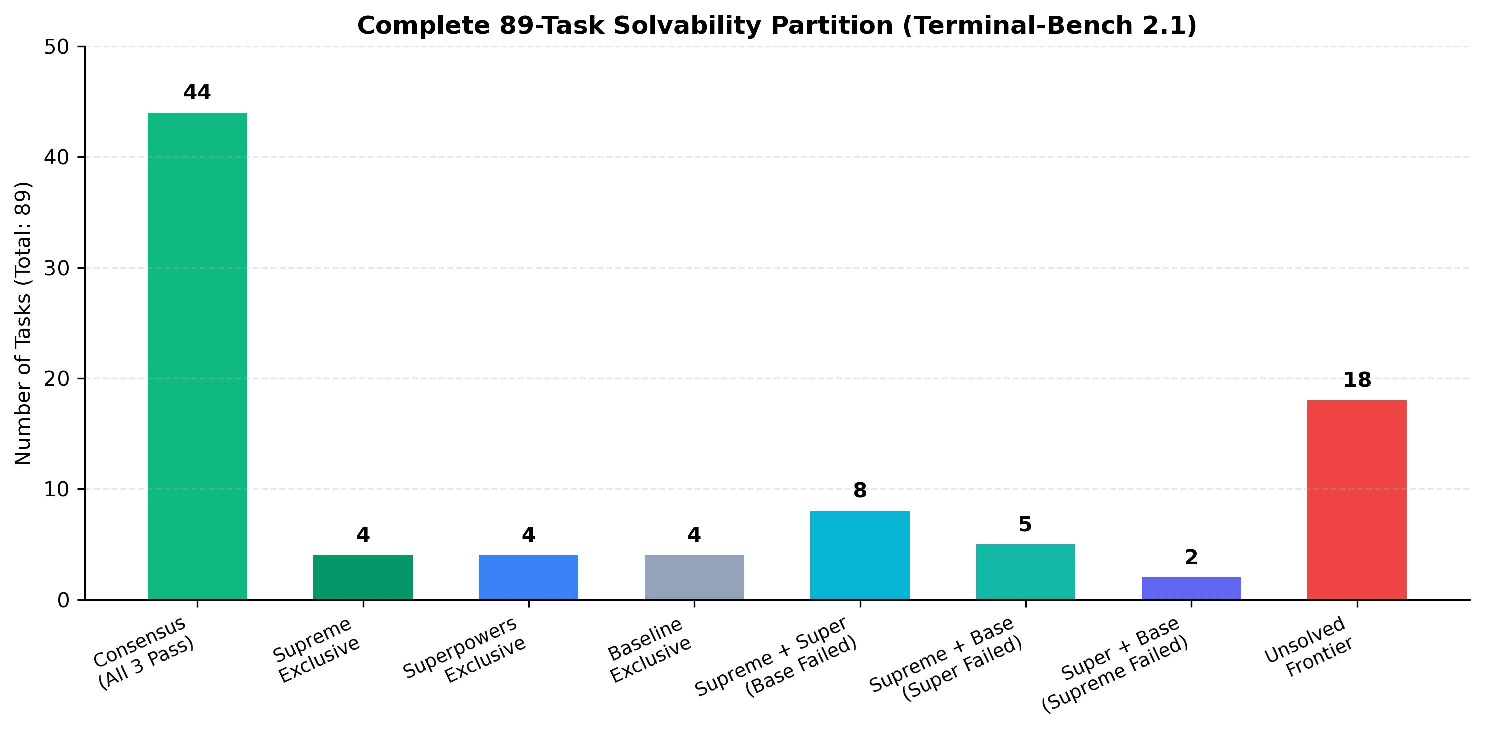
\includegraphics[width=0.48\textwidth]{figures/fig6_euler_venn_solvability_89tasks.pdf}
\caption{Domain versatility and task solvability partition. (Left) 5-Stack Polyglot performance radar. (Right) Complete 89-Task Mutual-Exclusion Partition across all eight mutually exclusive outcome subsets.}
\label{fig:polyglot_and_venn}
\end{figure*}

\subsection{Polyglot Domain Breakdown}
Table~\ref{tab:polyglot_stacks} summarizes pass rates across five engineering domains.

\begin{table}[h]
\centering
\caption{Performance Across 5 Engineering Stacks (Wilson 95\% CIs in brackets).}
\label{tab:polyglot_stacks}
\resizebox{\columnwidth}{!}{%
\begin{tabular}{lcccc}
\toprule
\textbf{Stack / Domain} & \textbf{Tasks} & \textbf{Supreme} & \textbf{Superpowers} & \textbf{Baseline} \\
\midrule
1. Low-Level Systems & 20 & \textbf{14 (70.0\%)} [48.1, 85.5] & 12 (60.0\%) [38.7, 78.1] & 13 (65.0\%) [43.3, 82.0] \\
2. SysAdmin \& DevOps & 15 & \textbf{13 (86.7\%)} [62.1, 96.3] & 11 (73.3\%) [48.1, 89.1] & 11 (73.3\%) [48.1, 89.1] \\
3. Software Engineering & 26 & \textbf{20 (76.9\%)} [57.9, 88.9] & \textbf{20 (76.9\%)} [57.9, 88.9] & 15 (57.7\%) [38.9, 74.5] \\
4. Esoteric \& Symbolic & 14 & 10 (71.4\%) [45.4, 88.3] & 9 (64.3\%) [38.8, 83.7] & \textbf{12 (85.7\%)} [60.1, 96.0] \\
5. ML \& Robotics & 14 & 4 (28.6\%) [11.7, 54.6] & \textbf{6 (42.9\%)} [21.4, 67.4] & 4 (28.6\%) [11.7, 54.6] \\
\midrule
\textbf{Total / Overall} & \textbf{89} & \textbf{61 (68.5\%)} [58.3, 77.2] & \textbf{58 (65.2\%)} [54.8, 74.3] & \textbf{55 (61.8\%)} [51.4, 71.2] \\
\bottomrule
\end{tabular}%
}
\end{table}

Due to sample sizes ($N=14$ to $26$), confidence intervals across stacks overlap substantially. Nonetheless, qualitative trends emerge:
\begin{itemize}
    \item \textbf{Low-Level Systems and SysAdmin}: Supreme demonstrated strong directional pass rates in C, Assembly, and OS administration, passing \texttt{gpt2-codegolf} (standalone C inference) and completing the 44-minute \texttt{install-windows-3.11} installation.
    \item \textbf{Esoteric \& Symbolic Tasks}: Unprompted Baseline achieved 85.7\% in Esoteric languages (Scheme, COBOL, LaTeX), outperforming both agent systems. Transcript inspection suggests that procedural guidance coincided with additional file-creation activity on these legacy toolchains, consistent with pre-trained model competency being sufficient for these task types without additional scaffolding.
\end{itemize}

\subsection{The Complete 89-Task Solvability Partition}
To examine task overlap without aggregation loss, Figure~\ref{fig:polyglot_and_venn} (Right) categorizes all 89 tasks into eight mutually exclusive subsets ($44 + 4 + 4 + 4 + 8 + 5 + 2 + 18 = 89$ tasks):
\begin{enumerate}
    \item \textbf{Consensus Passes ($N=44$)}: Solved by all three configurations.
    \item \textbf{Supreme Exclusive Wins ($N=4$)}: \texttt{fix-git}, \texttt{gpt2-codegolf}, \texttt{install-windows-3.11}, \texttt{tune-mjcf}.
    \item \textbf{Superpowers Exclusive Wins ($N=4$)}: \texttt{hf-model-inference}, \texttt{mailman}, \texttt{mteb-leaderboard}, \texttt{raman-fitting}.
    \item \textbf{Baseline Exclusive Wins ($N=4$)}: \texttt{build-pov-ray}, \texttt{gcode-to-text}, \texttt{qemu-alpine-ssh}, \texttt{regex-chess}.
    \item \textbf{Supreme + Superpowers Pass ($N=8$)}: Solved by both agent configurations but failed by Baseline (e.g., \texttt{build-cython-ext}, \texttt{cancel-async-tasks}, \texttt{fix-ocaml-gc}, \texttt{headless-terminal}, \texttt{large-scale-text-editing}, \texttt{merge-diff-arc-agi-task}, \texttt{video-processing}, \texttt{vulnerable-secret}).
    \item \textbf{Supreme + Baseline Pass ($N=5$)}: Solved by Supreme and Baseline but failed by Superpowers (\texttt{bn-fit-modify}, \texttt{circuit-fibsqrt}, \texttt{overfull-hbox}, \texttt{protein-assembly}, \texttt{rstan-to-pystan}).
    \item \textbf{Superpowers + Baseline Pass ($N=2$)}: Solved by Superpowers and Baseline but failed by Supreme (\texttt{largest-eigenval}, \texttt{model-extraction-relu-logits}).
    \item \textbf{Unsolved Frontier ($N=18$)}: Tasks unsolved by all configurations, including three tasks with verified upstream container bugs.
\end{enumerate}
One Superpowers-only pass (\texttt{mailman}) is verifier-graded (3/3 tests) with degraded agent telemetry from a stream-capture failure; it is retained as graded and flagged in the audit ledger.
This complete partition establishes that 71 of 89 tasks (79.8\%) were solved by at least one configuration, demonstrating complementary problem-solving strengths.



\section{Forensic Case Studies and Behavioral Dynamics}
\label{sec:case_studies}

To complement aggregate statistics, we examine individual execution transcripts that illuminate the behavioral mechanisms underlying the macro-level differences observed in Section~\ref{sec:results}. Four tasks across three distinct failure modes illustrate how architectural choices interact with specific problem classes.

\begin{figure*}[t]
\centering
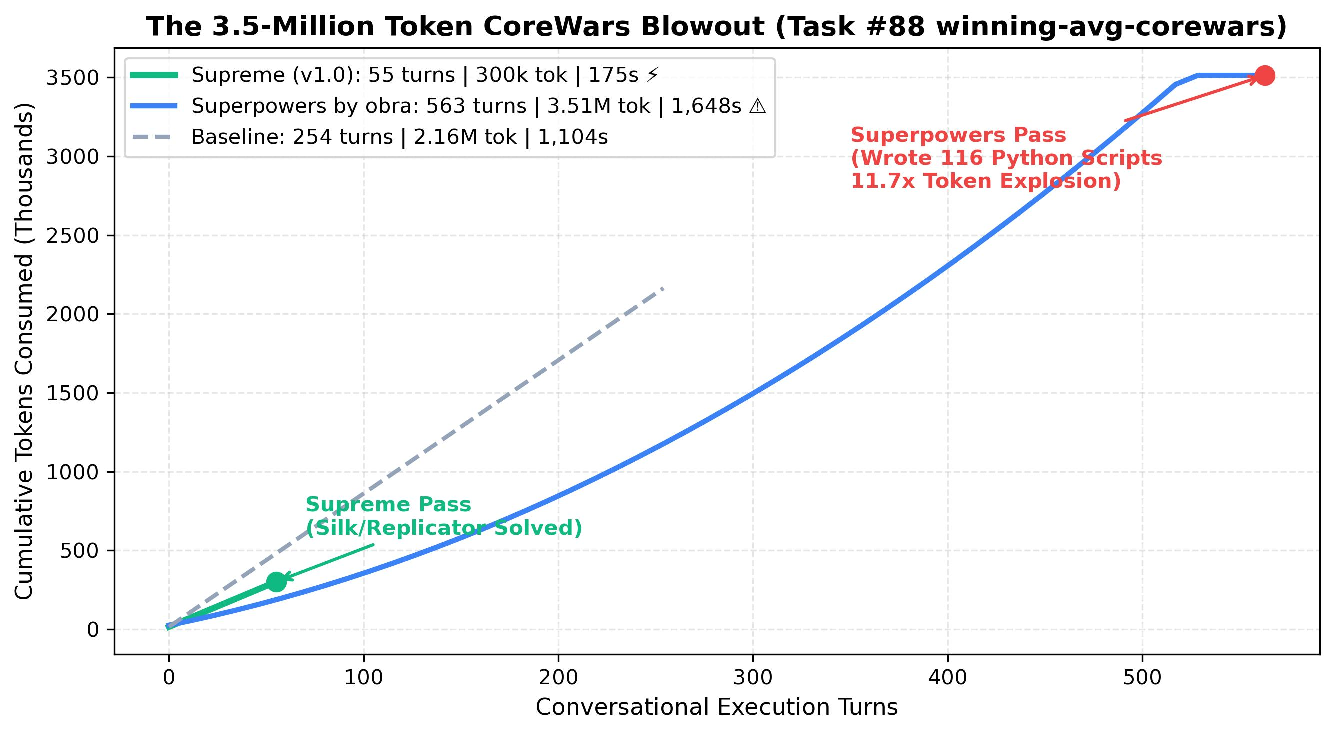
\includegraphics[width=0.48\textwidth]{figures/fig5_task88_corewars_trajectory.pdf}
\hfill
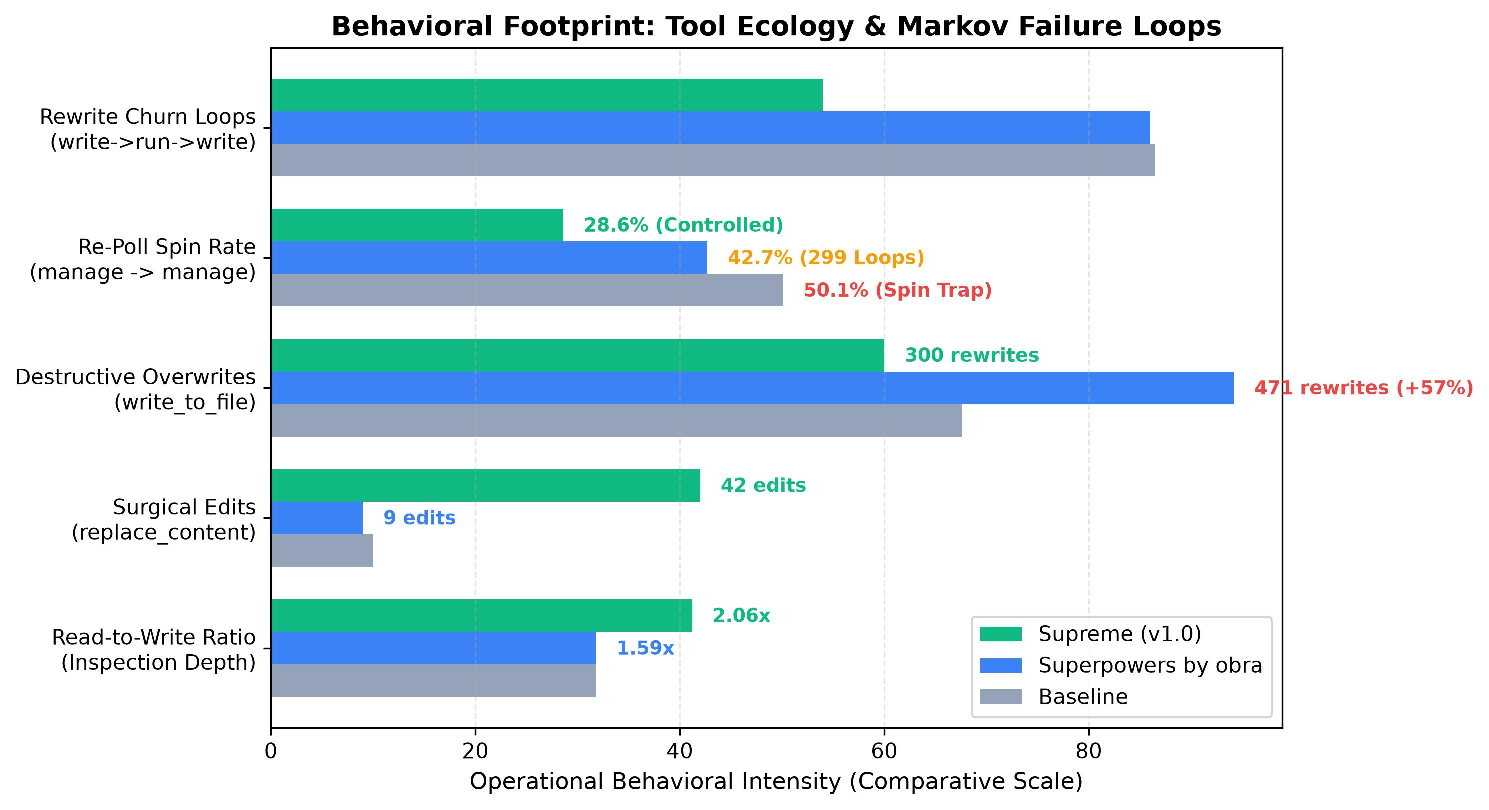
\includegraphics[width=0.48\textwidth]{figures/fig2_markov_tool_state_transitions.pdf}
\caption{Behavioral dynamics and tool interaction patterns. (Left) Cumulative token trajectory on Task \#88 (\texttt{winning-avg-corewars}), illustrating an extended parameter-search loop. (Right) Markov state transitions ($P(\text{Next} \mid \text{Current})$) comparing background task polling and file-editing strategies.}
\label{fig:trajectory_and_markov}
\end{figure*}

\subsection{Exploratory Scripting Loops (Task \#88: Redcode Simulation)}
In Task \#88 (\texttt{winning-avg-corewars}), agents were tasked with authoring a Redcode warrior in assembly meeting win thresholds against diverse archetypes in the MARS arena \cite{dewdney1984corewars}. The task specification defines a 3,600s execution limit ($T_{\text{limit}} = 3600$s).

As depicted in Figure~\ref{fig:trajectory_and_markov} (Left), this task produced the benchmark's widest divergence in computational expenditure:
\begin{itemize}
    \item \textbf{Supreme}: Inspected reference warriors, hypothesized that a Silk/Replicator archetype would dominate the arena pool, implemented the candidate warrior, verified win rates, and concluded in \textbf{175.0s}, \textbf{55 turns}, and \textbf{300,413 tokens}.
    \item \textbf{Superpowers by obra}: Entered an extensive parameter-search loop. Guided by iterative trial-and-error procedural guidance, the agent authored \textbf{116 separate Python exploration scripts}, repeatedly copying them into the container via \texttt{docker cp}, running battles, and accumulating \textbf{563 turns} across \textbf{1,648.7s} and \textbf{3,513,757 tokens} ($11.7\times$ token inflation for the identical pass).
\end{itemize}
This comparison highlights that on open-ended combinatorial tasks, procedural frameworks that encourage iterative scripting without strong stopping heuristics can lead to prolonged exploratory loops. This contrast does not represent a systematic throughput difference across all 89 tasks, where total billed token counts were comparable (34.52M vs.\ 34.30M), but rather illustrates the tail risk of unconstrained exploratory scripting on open-ended combinatorial problems.

\subsection{Markov Tool Transitions and Polling Dynamics}
Analysis of 15,779 sequential tool transitions ($P(\text{Next} \mid \text{Current})$) reveals key operational differences (Figure~\ref{fig:trajectory_and_markov}, Right):
\begin{itemize}
    \item \textbf{Background Task Polling}: When asynchronous background commands were active, Baseline exhibited a 50.1\% probability of immediately re-polling \texttt{manage\_task}; Superpowers exhibited 42.7\% (logging 299 triple-polling sequences (\texttt{manage} $\rightarrow$ \texttt{manage} $\rightarrow$ \texttt{manage})). Supreme's loop management protocol reduced this transition probability to 28.6\%, reducing uninformative polling turns.
    \item \textbf{File Modification Granularity}: Superpowers performed 471 full file overwrites (\texttt{write\_to\_file}) and 172 (\texttt{write} $\rightarrow$ \texttt{run} $\rightarrow$ \texttt{write}) churn cycles. Supreme utilized targeted line replacements (\texttt{replace\_file\_content}) more frequently (42 vs.\ 8). While higher usage of targeted editing reflects prompt compliance, it correlated with narrower modification blast radii: Supreme modified a mean of 2.60 unique files per task versus 3.79 on Superpowers.
\end{itemize}

\subsection{Physical Solver Optimization (Task \#85: MuJoCo Tuning)}
Task \#85 (\texttt{tune-mjcf}) required accelerating a MuJoCo physics simulation \cite{todorov2012mujoco} by $\ge 40\%$ without exceeding trajectory error bounds ($D \le 10^{-4}$). Supreme achieved an exclusive pass in 414.9s (81 tool calls, 436k tokens), attaining a \textbf{2.19$\times$ simulation speedup} with zero trajectory divergence ($D = 0.0000$). Baseline and Superpowers both failed to reach the speedup threshold ($0.99\times$ and $1.01\times$ speed ratios) due to speculative modifications of solver parameters.

\subsection{Long-Horizon Autonomy: Headless QEMU Installation}
In \texttt{install-windows-3.11} ($T_{\text{limit}} = 3600$s), agents were tasked with installing Windows 3.11 for Workgroups inside headless QEMU, partitioning virtual disks via \texttt{fdisk}, formatting FAT16, swapping floppy images, and installing network drivers. Supreme maintained autonomous multi-step execution across \textbf{2,648.7s (44.1 minutes)}, 307 turns, and 58,010 deliberation tokens to complete the installation. Superpowers and Baseline timed out or corrupted disk partition tables.

\subsection{Upstream Benchmark Harness Defects}
Forensic inspection identified three distinct upstream environmental failure modes spanning four tasks:
\begin{itemize}
    \item \texttt{prove-plus-comm} (Task \#64): Container metadata error caused immediate execution failure (\texttt{failed to chdir to cwd ("/app"): no such file or directory}) across all models.
    \item \texttt{caffe-cifar-10} (Task \#7): An unreleased package lock on \texttt{/var/lib/dpkg/lock-frontend} held by background PID 168 blocked package installations, causing a starvation timeout across all models.
    \item \textbf{Distributed PyTorch Infrastructure} (Tasks \#82--\#83): In Task \#82 (\texttt{torch-pipeline-parallelism}), the bare container lacked Python and curl with egress blocked; in Task \#83 (\texttt{torch-tensor-parallelism}), an unconstrained dynamic PyPI download of 2.85~GB CUDA wheels triggered a verifier timeout before test execution \cite{shoeybi2019megatron}.
\end{itemize}
Excluding the three environmental configuration defects (\texttt{prove-plus-comm}, \texttt{caffe-cifar-10}, and Task \#82) yields the $N=86$ adjusted cohort reported in Table~\ref{tab:master_scoreboard} (Supreme: 70.9\% [61/86]; Superpowers: 67.4\% [58/86]; Baseline: 64.0\% [55/86]). Excluding all four infrastructure-impaired tasks yields $N=85$ (Supreme: 71.8\% [61/85]; Superpowers: 68.2\% [58/85]; Baseline: 64.7\% [55/85]).



\section{Discussion and Context Economics}
\label{sec:discussion}

\begin{figure*}[t]
\centering
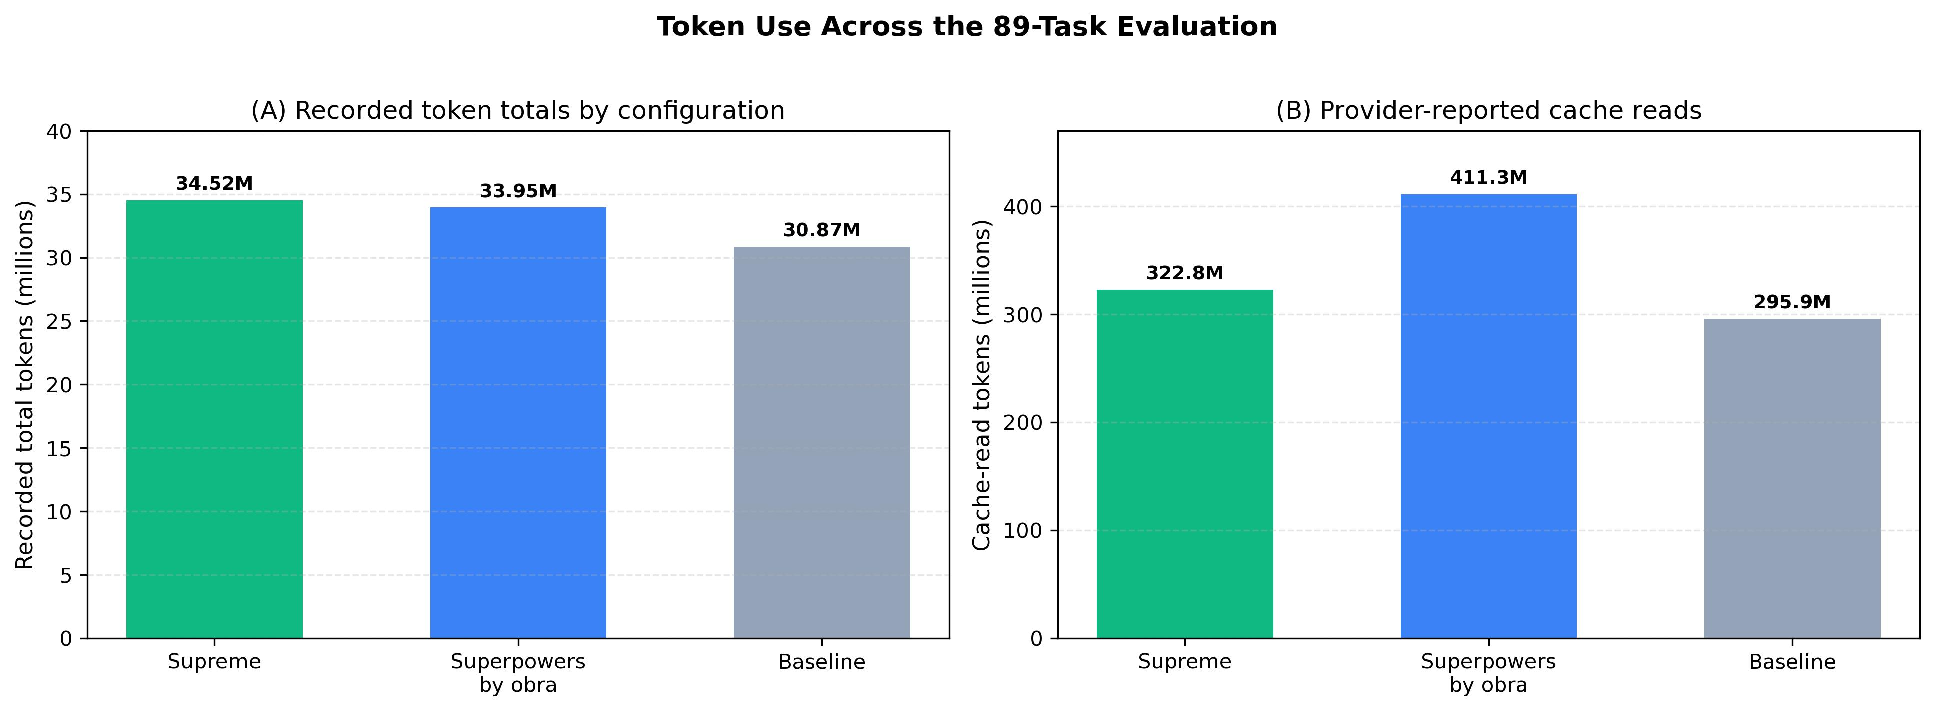
\includegraphics[width=\textwidth]{figures/fig4_token_usage_comparison.pdf}
\caption{Recorded token usage in the 89-task evaluation. (A) Recorded input-plus-output totals by configuration. (B) Provider-reported cache-read tokens, shown as a separate usage measure; the two panels are not additive components of one total.}
\label{fig:token_sinks}
\end{figure*}

\subsection{Context-Growth Dynamics and Multi-Turn Token Economics}
As illustrated in Figure~\ref{fig:token_sinks}, multi-turn agent execution exhibits distinctive context characteristics:
\begin{enumerate}
    \item \textbf{Input Share of Total Tokens}: For Supreme, input tokens comprised 90.5\% of recorded total tokens (31,232,870 / 34,521,410). This is an input-to-total ratio; it does not measure what share of input came from prior conversational history. In multi-turn runs, earlier conversation and tool outputs return as later-turn context, so initial prompt size alone does not describe full-trajectory input. Supreme's invariant header is approximately 7,000 tokens; Superpowers' initial discovery catalog is approximately 580 tokens and progressively loads procedural documents. These are different architectural layers: the comparison does not support describing Supreme as having the smaller initial context, nor does it quantify the complete skill-corpus sizes.
    \item \textbf{Observed Cache-Read Volume}: Provider-reported cache reads totaled \textbf{411,332,767 tokens} for Superpowers, 322,810,412 for Supreme, and 295,918,105 for Baseline \cite{google2026gemini36}. These are observed cache-read totals; this comparison does not isolate how much of the difference is attributable to dynamically loaded documentation.
    \item \textbf{Terminal Output in Tool Payloads}: Terminal stdout (including build logs and compiler output) represented 67.8\% of tool-payload tokens in the reported analysis. This points to output volume as a context-management consideration across configurations; it is not a measure of agent efficiency.
\end{enumerate}

\subsection{Financial Token Economics and Cost per Solved Task}
Table~\ref{tab:cost_economics} reports modeled API costs across the 267 evaluations under two rate schedules: the Gemini list-price reference (\$0.75 / M input, \$3.75 / M output) and the recorded OpenRouter rates (\$0.5598 / M input, \$3.745 / M output). These are rate-based estimates, not reported transaction charges.

\begin{table}[h]
\centering
\caption{Recorded token totals and rate-based cost estimates for the 267-evaluation study.}
\label{tab:cost_economics}
\resizebox{\columnwidth}{!}{%
\begin{tabular}{lccc}
\toprule
\textbf{Economic Dimension} & \textbf{Supreme} & \textbf{Superpowers} & \textbf{Baseline} \\
\midrule
Input Tokens ($T_{\text{in}}$) & 31.23M & 30.71M & \textbf{27.71M} \\
Output Tokens ($T_{\text{out}}$) & 3.29M & 3.25M & \textbf{3.16M} \\
Deliberation Tokens ($T_{\text{think}}$) & 1.83M & \textbf{1.71M} & 1.77M \\
Recorded Total Tokens (Input + Output) & 34.52M & 33.95M & \textbf{30.87M} \\
Cache Read Tokens ($T_{\text{cache}}$) & 322.8M & 411.3M & \textbf{295.9M} \\
\midrule
Modeled Total (List-Price Rates) & \$35.76 & \$35.21 & \textbf{\$32.62} \\
Modeled Cost / Successful Task (List) & \textbf{\$0.586} & \$0.607 & \$0.593 \\
\midrule
Modeled Total (OpenRouter Rates) & \$29.80 & \$29.35 & \textbf{\$27.33} \\
Modeled Cost / Attempted Task (OpenRouter) & \$0.335 & \$0.330 & \textbf{\$0.307} \\
Modeled Cost / Successful Task (OpenRouter) & \textbf{\$0.489} & \$0.506 & \$0.497 \\
Modeled Hard-Task Cost / Successful Task ($N=30$) & \$0.680 & \$0.730 & \textbf{\$0.645} \\
\bottomrule
\end{tabular}%
}
\end{table}
\par\smallskip{\footnotesize\noindent\emph{Note:} Component values are rounded independently; deliberation tokens are included in output and shown separately.\par}\smallskip

Across all 89 tasks, the rate-based cost estimates and outcomes present a three-layer economic portrait. Under the OpenRouter-rate model, Baseline had the lowest modeled total cost (\$27.33), followed by Superpowers (\$29.35) and Supreme (\$29.80). Baseline also had the lowest modeled cost per attempted task (\$0.307), followed by Superpowers (\$0.330) and Supreme (\$0.335). These modeled cost advantages coincide with Baseline's lower recorded token total (30.87M vs.\ 34.52M for Supreme), but also with its lower task completion (55/89 vs.\ 61/89).

Cost per successful task is a composite measure combining modeled total cost with the number of successful tasks; it is not a separately observed charge. On this measure, Supreme had the lowest modeled cost per successful task under the recorded OpenRouter rates (\$0.489), approximately 3.4\% below Superpowers (\$0.506), while completing three additional tasks (61 vs.\ 58). Baseline was \$0.497. The ranking is unchanged under both the list-price and OpenRouter-rate scenarios in Table~\ref{tab:cost_economics}.

On the Hard task subset ($N=30$), the cost-per-successful-task ranking reverses: Baseline achieved the lowest cost per successful Hard task (\$0.645), followed by Supreme (\$0.680) and Superpowers (\$0.730). Supreme simultaneously achieved the highest Hard-task completion rate (66.7\% [20/30] vs.\ 56.7\% [17/30] for Baseline and 53.3\% [16/30] for Superpowers), representing a genuine trade-off of superior Hard-task coverage at moderately higher cost per successful Hard solve compared to Baseline.

\subsection{Practical Design Implications for Agent Systems}
The evaluated configurations suggest three practical design considerations:
\par\textbf{Static Invariant Principles}: Static placement of invariant engineering principles can avoid mid-turn documentation retrieval while maintaining consistent behavioral constraints across turns.
\par\textbf{Loop Termination Heuristics}: Explicit iteration thresholds and hypothesis-checking gates help limit prolonged exploratory scripting on open-ended combinatorial problems.
\par\textbf{Targeted Line Edits}: Surgical diff tools (\texttt{replace\_file\_content}) correlate with reduced collateral modifications compared to whole-file rewrites.

\subsection{Threats to Validity and Limitations}
\textbf{Single Foundation Model}: All evaluations used Gemini 3.6 Flash High. Model-specific reasoning and tool policies may interact with prompt architecture; findings may not generalize across model families without multi-model replication.
\par\textbf{Single Run per Task}: Each task was evaluated with one run per configuration at $\tau=0.0$ (267 container runs, $\approx 50$ compute hours). While $\tau=0.0$ minimizes sampling variance, multi-seed replication is needed to measure run-to-run stability.
\par\textbf{Coupled Structure and Content}: Supreme and Superpowers differ in structure (static vs.\ dynamic) and content (constitutional axioms vs.\ TDD workflows). Controlled ablations isolating delivery mechanism from content remain future work.
\par\textbf{Prompt Freezing}: The Supreme constitutional prompt was frozen prior to benchmark execution; no prompt adjustments were made based on benchmark task failures.

\vspace{-0.3em}
\section{Conclusion}
\label{sec:conclusion}
Across the 89-task Terminal-Bench 2.1 evaluation (267 isolated container runs), the complete Supreme configuration recorded the highest task-completion rate (61/89, 68.5\%), the lowest aggregate wall-clock time (15.15\,h, 17.2\% below Superpowers), and the lowest modeled cost per successful task under recorded OpenRouter rates (\$0.489 vs.\ \$0.506 for Superpowers and \$0.497 for Baseline). Baseline had the lowest modeled absolute cost (\$27.33) and the lowest recorded token total (30.87M); Supreme's recorded total was 34.52M and Superpowers' was 33.95M. Supreme also recorded a directional lead on Hard tasks (20/30 vs.\ 16/30 for Superpowers and 17/30 for Baseline; paired McNemar $p = 0.22$). Aggregate completion differences were not statistically distinguishable under paired McNemar tests ($p > 0.05$). These results compare complete configurations with different guidance content and delivery mechanisms; they do not establish that static or dynamic delivery alone caused the observed differences. The evaluation provides an empirical baseline for this skill and benchmark; future work should replicate across model families and use controlled ablations to isolate design factors.



{\small
\bibliographystyle{plain}
\bibliography{references}
}


\end{document}
